\documentclass[titlepage = firstcover]{scrartcl}
\usepackage[aux]{rerunfilecheck}
\usepackage{fontspec}
\usepackage[main=ngerman, english, french]{babel}

% mehr Pakete hier
\usepackage{expl3}
\usepackage{xparse}
\usepackage{pdfpages}
\usepackage{csvsimple}
\usepackage{pgfplotstable}

%Mathematik------------------------------------------------------
\usepackage{amsmath}   % unverzichtbare Mathe-Befehle
\usepackage{amssymb}   % viele Mathe-Symbole
\usepackage{mathtools} % Erweiterungen für amsmath
\usepackage[
  math-style=ISO,    % \
  bold-style=ISO,    % |
  sans-style=italic, % | ISO-Standard folgen
  nabla=upright,     % |
  partial=upright,   % /
]{unicode-math}% "Does exactly what it says on the tin."

% Laden von OTF-Mathefonts
% Ermöglich Unicode Eingabe von Zeichen: α statt \alpha

\setmathfont{Latin Modern Math}
%\setmathfont{Tex Gyre Pagella Math} % alternativ zu Latin Modern Math
\setmathfont{XITS Math}[range={scr, bfscr}]
\setmathfont{XITS Math}[range={cal, bfcal}, StylisticSet=1]

\AtBeginDocument{ % wird bei \begin{document}
  % werden sonst wieder von unicode-math überschrieben
  \RenewDocumentCommand \Re {} {\operatorname{Re}}
  \RenewDocumentCommand \Im {} {\operatorname{Im}}
}
\usepackage{mleftright}
\setlength{\delimitershortfall}{-1sp}

%Sprache----------------------------------------------------------
\usepackage{microtype}
\usepackage{xfrac}
\usepackage[autostyle]{csquotes}    % babel
\usepackage[unicode, pdfusetitle]{hyperref}
\usepackage{bookmark}
\usepackage[shortcuts]{extdash}
%Einstellungen hier, z.B. Fonts
\usepackage{booktabs} % Tabellen
\usepackage{a4}
\usepackage{float}
%Subfiguren
\usepackage{graphicx}
\usepackage{grffile}
\usepackage{subcaption}
\usepackage[section, below]{placeins}

\setlength{\parindent}{0pt}


\title{Biegung elastischer Stäbe}
\author{
  David Gutnikov \\
  \href{mailto:david.gutnikov@edu.udo}{david.gutnikov@edu.udo} \and
  Lasse Sternemann \\
  \href{mailto:lasse.sternemann@edu.udo}{lasse.sternemann@edu.udo}}
\date{Durchführung am 26.11.19}

\begin{document}
    \maketitle
    \tableofcontents
    \newpage
    
    \section{Zielsetzung}
      Es sollen für verschiedene Stäbe die Proportionalitätskoeffizienten (Elastizitätsmodul) zwischen ausreichend kleinen Auslenkungen des Stabes und der auf ihn ausgeübten Spannung bestimmt werden.

    \section{Theorie}
      \subsection{Elastizitätsmodul}
        Wenn Kräfte auf einen elastischen Körper wirken, verformt sich dieser, wie in Abbildung \ref{fig:verformung}
        zu sehen ist. Meistens werden diese Kräfte pro Fläche angegeben, was als Spannung bezeichnet wird.
        Diese Spannungen haben einen linearen Zusammenhang zu den durch sie verursachten, relativen Auslenkungen am
        Körper (Auslenkung relativ zur Länge des Körpers), sofern sie ausreichend klein sind.
        Der Proportionalitätskoeffizient dieser Abhängigkeit ist der Elastizitätsmodul. Jedes Material besitzt ein
        eigenes Elastizitätsmodul, welches als Materialkonstante in verschiedenen Fachbereichen Anwendung findet.
        \begin{figure}[h]
          \centering
          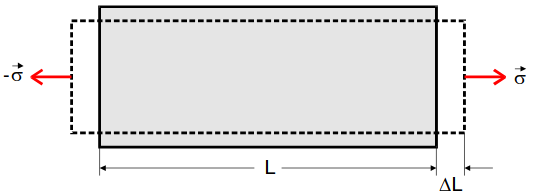
\includegraphics[width=0.75\linewidth]{Verformung.png}
          \caption{Der Körper wird durch $\sigma$ verformt und erfährt eine Ausdehnung von $\Delta L$. [1, S.1]}
          \label{fig:verformung}
        \end{figure}
        
        Die Formel bzw. das \glqq Hook'sche Gesetz\grqq{} sieht wie folgt aus mit der Auslenkung $\Delta L$ und der Länge des Körpers $L$:
        \begin{equation*}
          \sigma = E \cdot \frac{\Delta L}{L}
        \end{equation*}
        
        \subsection{Biegung eines einseitig eingespannten Stabes}
          Wie in Abbildung \ref{fig:theorieEins} zu sehen ist, wird der Stab durch die senkrecht zu ihm angreifende Kraft $F$ um $D$ 
          ausgelenkt. Die Auslenkung kommt zustande, indem der Stab sich durch das äußere Drehmoment biegt, bis die 
          inneren Normalspannungen ein Kräftegleichgewicht erzeugen und der Stab in der zugehörigen Auslenkung verbleibt.
          Diese Auslenkung hängt vom Abstand zum Befestigungspunkt $x$, dem Elastizitätsmodul des Körpermaterials $E$, 
          dem Flächenträgheitsmoment $I$ und der Länge des Körper s$L$, sowie der angreifenden Kraft $F$ ab. Dieser 
          Zusammenhang ist in Formel \eqref{eqn:formelEins} dargestellt:
          \begin{equation}
            D(x) = \frac{F}{2EI} \cdot \Bigl(Lx^2 - \frac{x^3}{3}\Bigr)
            \label{eqn:formelEins}
          \end{equation}

          \begin{figure}[h]
            \centering
            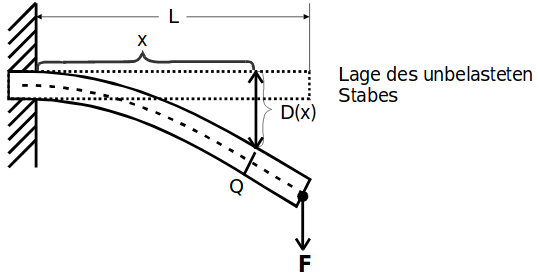
\includegraphics[width=0.75\linewidth]{Einseitig_Theorie.png}
            \caption{Der Stab wird einseitig eingespannt und an einer Seite ein Gewicht angehängt. [1, S.2]}
            \label{fig:theorieEins}
          \end{figure}
      
        \subsection{Biegung eines zweiseitig eingespannten Stabes}
          Wie in \ref{eqn:formelZweis} zu sehen ist, wird in der Mitte zwischen den Auflagepunkten eine senkrechte Kraft an
          den Stab angelegt. Die anliegende Kraft wird auf die beiden Auflagepunkte übertragen und erzeugt auch hier nach 
          dem obrigen Prinzip eine Auslenkung. Diese ist von den selben Größen wie Formel \eqref{eqn:formelEins} abhängig, 
          unterscheidet sich jedoch um den Faktor 1/24. Demnach ergibt sich für die zweiseitige Auflage Formel 
          \eqref{eqn:formelZweis}:
          \begin{equation}
            D(x) = \frac{F}{48EI} \cdot \Bigl(3L^2x - 4x^3\Bigr)
            \label{eqn:formelZweis}
          \end{equation}

          \begin{figure}[h]
            \centering
            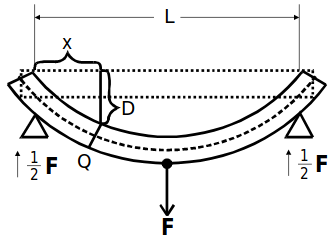
\includegraphics[width=0.5\linewidth]{Zweiseitig_Theorie.png}
            \caption{Der Stab wird einseitig eingespannt und an einer Seite ein Gewicht angehängt. [1, S.5]}
            \label{fig:theorieZwei}
          \end{figure}
      

    \section{Versuchsdurchführung}
      Zur Bestimmung des Elastizitätsmoduls der Stabmaterialien werden Gewichte an dem Stab angebracht und daraufhin dessen Auslenkung abhängig von der Entfernung
      zum Angriffspunkt des Gewichts gemessen. Es werden zwei Stäbe verwendet, von denen einer einen runden Querschnitt und der andere einen rechteckigen hat. Beide
      Stäbe werden in zwei Positionen eingespannt und gemessen. Zum einen werden sie nur an einem Auflagepunkt eingespannt und das Gewicht möglichst weit davon entfernt
      angebracht. Dieser Aufbau ist in Abbildung \ref{fig:theorieEins} zu sehen. Bei dem zweiten, in Abbildung \ref{fig:formelZweis} zu sehenden Aufbau, liegt der Stab auf zwei Auflagepunkten und das
      Gewicht greift in der Mitte der beiden Auflagepunkte an.\newline

      Zur Messung der Auslenkung werden Messuhren wie in Abbildung \ref{fig:fotoUhr} verwendet. Diese bestehen aus einem, an einer Feder befestigten, Messtaster und einer runden Skala. Wenn der 
      Messtaster eingedrückt wird, wird die Distanz auf der Rundskala, die von 0,01 bis 10 Millimeter geht, angezeigt. Mit diesen Messuhren wird vor Beginn der
      Messung der Auslenkung des Stabes über den unausgelenkten Stab gefahren, um die Auslenkung in der Ruhelage zu messen. Dies ist notwendig, da die Stäbe 
      bereits sehr of ausgelenkt worden sind und nie wieder in die ehemalige gerade Form zurückgekehrt sind. Nachdem auf diese Weise, die Ruheauslenkung 
      festgestellt worden ist, wird das Gewicht angehangen und erneut mit den Messuhren über den Stab gefahren. Dabei werden in Abständen von 3 cm die realtiven 
      Auslenkungen gemessen. Im Nachhinein werden die Ruheauslenkungen von den realtiven Auslenkungen abgezogen, um die tatsächliche Auslenkung des Stabes zu
      messen. Da die Messuhr bei zweiseitiger Einspannung in der Mitte blockiert wird, muss in diesem Fall mit zwei verschiedenen Messuhren gemessen werden. Dies
      kann zu unterschieden in den Messergebnissen führen, da bei unserem Experiment besonders eine der Uhren sehr unzuverlässige Werte lieferte.
      
      \begin{figure}[h]
        \centering
        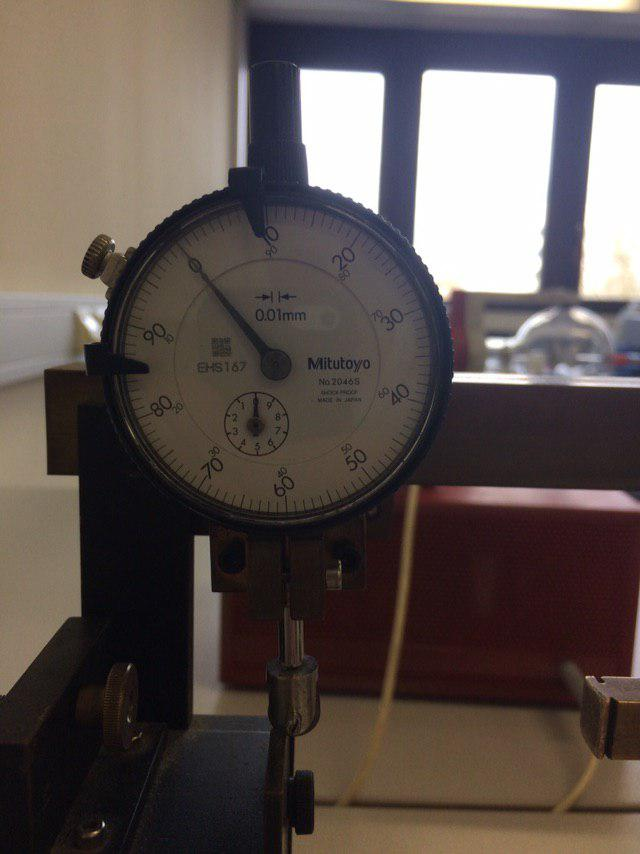
\includegraphics[width=0.25\linewidth]{Messuhr.jpg}
        \caption{Zu sehen ist eine der mechanischen Messuhren, die zur Bestimmung der Auslenkung genutzt worden ist. Sie ist auf 0,01mm genau und kann Längen bis zu 10mm messen.}
        \label{fig:fotoUhr}
      \end{figure}   
      
      \FloatBarrier

    \newpage

    \section{Auswertung}
      Für das Experiment wurde ein Stab mit rechteckiger Querschnittfläche der Länge $l_e = 0,639 m$, der langen Seite der Grundfläche $b = 0,0122 m$, der kurzen Seite der
      Grundfläche $a = 0,011 m$ und der Masse $m_e = 0,605 kg$ und ein runder Stab mit der Länge $l_r = 0,6 m$, dem Radius $r = 0,0044 m$ und der Masse $m_r = 0,3655 kg$ verwendet. Zum späteren 
      Ermitteln des Elastizitätsmoduls müssen zunächst die Flächenträgheitsmomente der Stäbe berechnet werden. Dies erfolgt über die unten folgenden Formeln.
      \begin{gather}
        I_e = \frac{ab^3}{12} = 1,6645 \cdot 10^{-9} m⁴\\
        I_r = \frac{\pi r^4}{4} = 2,94375 \cdot 10^{-10} m⁴
        \label{eqn:Flächenträg}
      \end{gather}
      Um mit den Messwerten die Elastizitätsmodule zu bestimmen wird von einer linearen Regression gebrauch gemacht. Aus ihrer Steigung lässt sich nach Formel
      \ref{eqn:linregress} das Elastizitätsmodul bestimmen. In den Gleichung für den Elastizitätsmodul steht L für die Länge vom
      Einspannpunkt zum Gewicht bzw. vom einen Auflagepunkt zum Anderen. DIe Kraft $F$ resultiert aus der angehängten Masse $m$.
      Bei zweiseitiger Einspannung werden für $x$, die $x_{rel}-Werte$ aufgetragen.
      \begin{align}
        D(x) &= \frac{F}{48EI} &\cdot &\Bigl(3L^2x - 4x^3\Bigr) & \\
        \label{eqn:linregresskomplett}
        D(x) &= \frac{F}{2EI} &\cdot &\Bigl(Lx^2 - \frac{x^3}{3}\Bigr) & \\
          y  &= m &\cdot &x &+ b
        \label{eqn:linregress}
      \end{align}
      \subsection{Eckiger Stab}
        Um später einen Referenzwert zum gemessenen Elastizitätsmodul zu haben, wird die Dichte des Körpers mit Formel \ref{eqn:DichteEck} berechnet.
        \begin{equation}
          \rho = \frac{m_e}{a b l_e} = 7,055 \frac{g}{cm^3}
          \label{eqn:DichteEck}
        \end{equation}
        Auch wenn sich die Dichte des Stabes um circa 21 \% von der Literaturdichte von Kupfer [1, S.1509] (8,92 g/cm³) unterscheidet, lässt sich aufgrund der
        markanten Farbe des Stabes vermuten, dass es sich um einen Kupferstab handelt.    
        \begin{table}[h]
          \centering
          \caption{Messwerte des eckigen, einseitig eingespannten Stabes.
                   $x$ ist der Abstand vom Einspannpunkt,
                   $D_0(x)$ ist die Auslenkung ohne Krafteinwirkung,
                   $D_a(x)$ ist die Auslenkung mit Krafteinwirkung,
                   $D(x)$ ist die tatsächliche Auslenkung, also die Differenz von $D_a$ und $D_0$.}
          \label{tab:tabEeins}
          \begin{tabular}{c c c c}
            \toprule
            {$x$ [m]} & {$D_0(x)$ [$10^{-3}m$]} & {$D_a(x)$ [$10^{-3}m$]} & {$D(x)$ [$10^{-3}m$]}\\
            \midrule
            0.03 & 0.07 & 0.17 & 0.10\\
            0.06 & 0.09 & 0.39 & 0.30\\
            0.09 & 0.11 & 0.57 & 0.46\\
            0.12 & 0.15 & 0.86 & 0.75\\
            0.15 & 0.17 & 1.20 & 1.03\\
            0.18 & 0.22 & 1.63 & 1.47\\
            0.21 & 0.24 & 1.97 & 1.73\\
            0.24 & 0.10 & 2.40 & 2.30\\
            0.27 & 0.09 & 2.80 & 2.71\\
            0.30 &-0.05 & 3.26 & 3.31\\
            0.33 &-0.11 & 3.74 & 3.85\\
            0.36 &-0.21 & 4.23 & 4.44\\
            0.39 &-0.25 & 4.77 & 5.02\\
            0.42 &-0.31 & 5.33 & 5.64\\
            0.45 &-0.33 & 5.89 & 6.22\\
            \bottomrule            
          \end{tabular}
        \end{table}

        \begin{figure}[h]
          \centering
          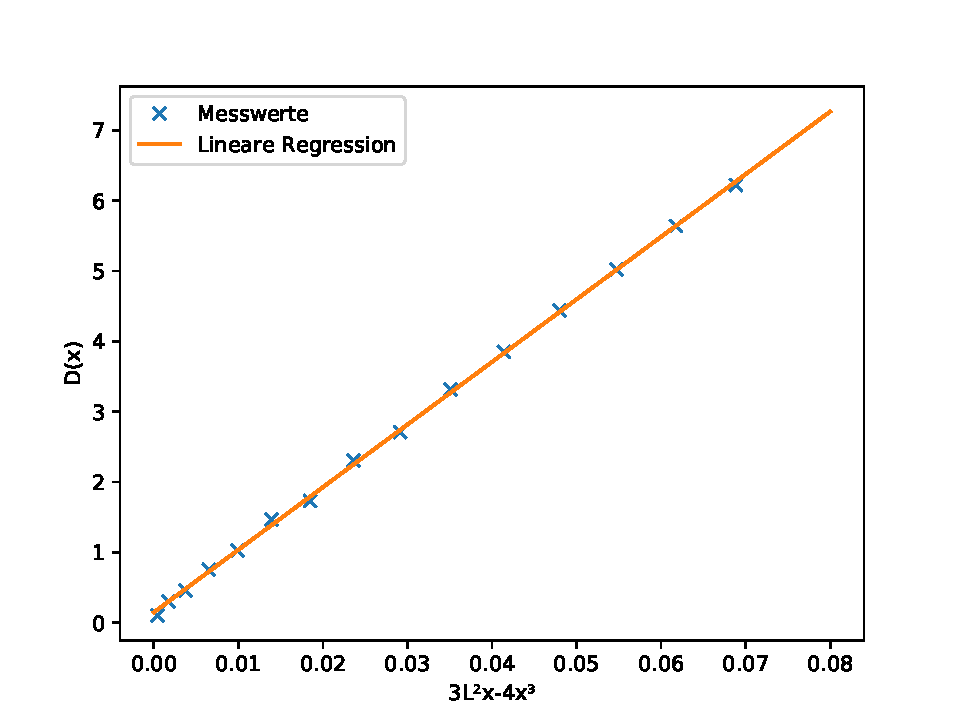
\includegraphics[width=0.7\linewidth]{eeins.pdf}
          \caption{In der Grafik sind die Auslenkungen D gegen Lx²-x³/3 aufgetragen. Durch diese Wertepaare wurde zudem per linearer Regression eine Ausgleichsgerade gelegt. Deren Steigung beträgt 0,08901088 und deren y-Achsenabschnitt 0,00014607.}
          \label{fig:graphEeins}
        \end{figure}

        Durch Umstellen von Gleichung \ref{eqn:linregresskomplett} bei $x = 0$ lässt sich das Elastizitätsmodul einfach berechnen. Der Fehler des Elastizitätsmoduls stammt aus der Gauß´schen 
        Fehlerfortpflanzung des Fehlers der Steigung aus der linearen Regression. $m$ beträgt 2,3679 kg und $L$ beträgt 0,49 m.
        \begin{equation}
          \Delta E = \frac{mg}{m^2 I n} \cdot \Delta m \quad \text{mit n = 2 bzw. 48}
          \label{eqn:Gauß}
        \end{equation}
        \begin{equation*}
          E_1 = \frac{mg}{2mI} = 96,3950 \pm 5,9635 GPa \quad \text{mit } \Delta a = \pm 5,9636 \cdot 10^{-4} Pa
        \end{equation*}

        \newpage

        \begin{table}[h]
          \centering
          \caption{Messwerte des eckigen, zweiseitig eingespannten Stabes.
                   $x$ ist der Abstand vom rechten Einspannpunkt,
                   $D_0(x)$ ist die Auslenkung ohne Krafteinwirkung,
                   $D_a(x)$ ist die Auslenkung mit Krafteinwirkung,
                   $D(x)$ ist die tatsächliche Auslenkung, also die Differenz von $D_a$ und $D_0$,
                   $x_{rel}$ ist der Abstand zum jeweils näheren Einspannpunkt.}
          \label{tab:tabEzwei}
          \begin{tabular}{c c c c c}
            \toprule
            {$x$ [m]} & {$D_0(x)$ [$10^{-3}m$]} & {$D_a(x)$ [$10^{-3}m$]} & {$D(x)$ [$10^{-3}m$]} & {$x_{rel}$ [m]}\\
            \midrule
            0.03 &  0.05 &  0.17 & 0.12 & 0.03\\
            0.06 &  0.10 &  0.31 & 0.21 & 0.06\\
            0.09 &  0.16 &  0.46 & 0.30 & 0.09\\
            0.12 &  0.25 &  0.63 & 0.38 & 0.12\\
            0.15 &  0.29 &  0.63 & 0.38 & 0.15\\
            0.18 &  0.40 &  0.94 & 0.54 & 0.18\\
            0.21 &  0.38 &  0.96 & 0.56 & 0.21\\
            0.24 &  0.41 &  1.02 & 0.61 & 0.24\\
            0.30 & -0.04 &  0.74 & 0.78 & 0.24\\
            0.33 & -0.15 &  0.62 & 0.77 & 0.21\\
            0.36 & -0.26 &  0.45 & 0.71 & 0.18\\
            0.39 & -0.36 &  0.28 & 0.64 & 0.15\\
            0.42 & -0.45 &  0.10 & 0.55 & 0.12\\
            0.45 & -0.56 & -0.12 & 0.44 & 0.09\\
            0.48 & -0.65 & -0.33 & 0.32 & 0.06\\
            0.51 & -0.77 & -0.55 & 0.22 & 0.03\\
            0.54 & -0.92 & -0.70 & 0.22 & 0.01\\
            \bottomrule            
          \end{tabular}
        \end{table}
  
        \newpage

        \begin{figure}[h]
          \centering
          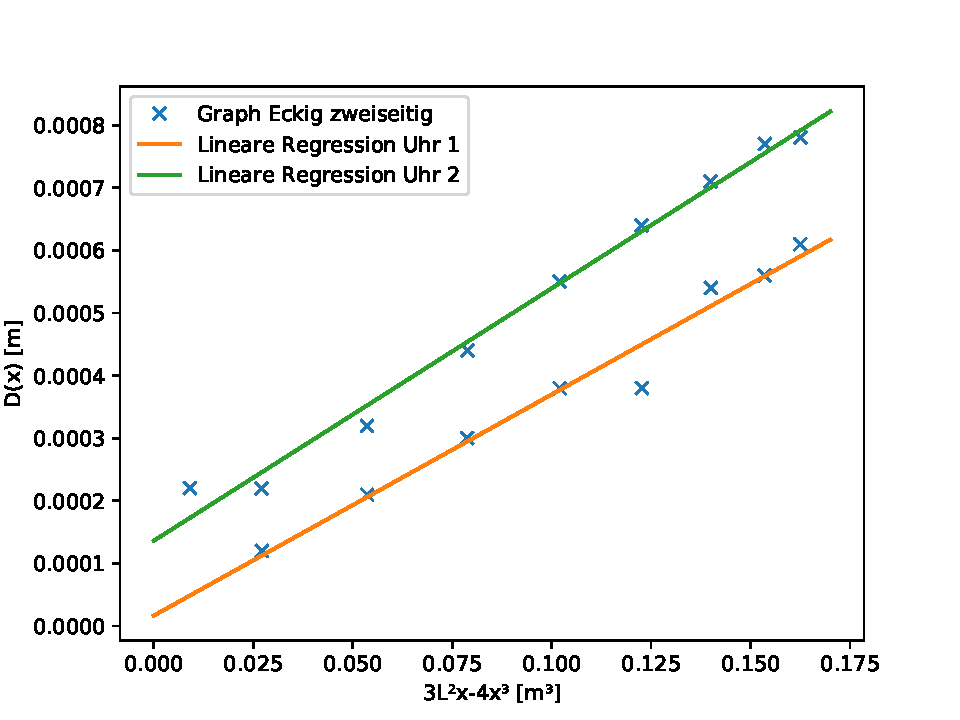
\includegraphics[width=0.7\linewidth]{ezwei.pdf}
          \caption{In der Grafik sind die Auslenkungen D gegen Lx²-x³/3 aufgetragen. Durch diese Wertepaare wurde zudem per linearer Regression zwei Ausgleichsgerade gelegt. Es wurden zwei Ausgleichsgeraden generiert, da die zwei Uhren stark unterschiedlich gemessen haben. Die Gerade von Uhr 1 hat die Steigung $3,53205921\cdot10^{-3}$ und den y-Achsenabschnitt $1,65755043\cdot10^{-5}$, die von Uhr 2 die Steigung $4,03285\cdot10^{-3}$ und den y-Achsenabschnitt $0.13614\cdot10^{-3}$.}
          \label{fig:graphEzwei}
        \end{figure}

        Auch hier lässt sich das Elastizitätsmodul durch Umstellen von Gleichung \ref{eqn:linregresskomplett} bei $x = 0$ nach E berechnen. Diese mal stammt der Fehler aus der Gauß´schen 
        Fehlerfortpflanzung des gemittelten Fehlers der Steigungen aus den zwei linearen Regression, die aufgrund der unterschiedlichen Uhren durchgeführt 
        worden sind. Die Masse entspricht der bei einseitiger Einspannung und $L$ beträgt 0,55 m.
        \begin{equation*}
          \Delta a = (\Delta a_1 + \Delta a_2) \cdot \frac{1}{2} = 2,0632 \cdot 10^{-4}
        \end{equation*}
        \begin{equation*}
          E_2 = \frac{mg}{2mI} = 76,8383 \pm 4,1913 GPa \quad \text{mit } \Delta a = \pm 2,0632 \cdot 10^{-4}
        \end{equation*}

        Beim Vergleich der beiden Elastizitätsmodule fällt auf, dass $E_2$ um 20,3 \% von $E_1$ abweicht. 
        Währenddessen ist der Literaturwert $E_{Cu,Lit} = 100$GPa [4]. $E_1$ weicht davon um 3,74 \% und $E_2$ um 30,14 \% ab.

        \FloatBarrier

      \newpage

      \subsection{Runder Stab}
      \begin{table}[h]
        \centering
        Wieder wird über das Volumen und die Masse des Stabes die Dichte zur Identifizierung des Materials berechnet.
        \begin{equation*}
          \rho = \frac{m_r}{\pi r^2 l_r} = 10,0157 \frac{g}{cm^3}
        \end{equation*}
        Auch hier scheint die graue Farbe bereits Rückschluss auf das Metall Eisen ziehen lassen. Da die gemessene Dichte auch nur 22,6 Prozent von der 
        Literaturdichte (7,85 g/cm³) [4] abweicht, gehen wir von einem eisernen Stab aus. 
        \caption{Messwerte des runden, einseitig eingespannten Stabes wie in Tabelle \ref{tab:tabEeins}.}
        \label{tab:tabReins}
        \begin{tabular}{c c c c}
          \toprule
          {$x$ [m]} & {$D_0(x)$ [$10^{-3}m$]} & {$D_a(x)$ [$10^{-3}m$]} & {$D(x)$ [$10^{-3}m$]}\\
          \midrule
          0.03 &-0.01 & 0.08 & 0.09\\
          0.06 &-0.14 & 0.06 & 0.20\\
          0.09 &-0.28 & 0.10 & 0.38\\
          0.12 &-0.39 & 0.17 & 0.56\\
          0.15 &-0.52 & 0.29 & 0.81\\
          0.18 &-0.60 & 0.49 & 1.09\\
          0.21 &-0.76 & 0.63 & 1.39\\
          0.24 &-0.84 & 0.89 & 1.73\\
          0.27 &-0.93 & 1.15 & 2.08\\
          0.30 &-1.05 & 1.43 & 2.48\\
          0.33 &-1.13 & 1.73 & 2.86\\
          0.36 &-1.22 & 2.06 & 3.28\\
          0.39 &-1.31 & 2.42 & 3.71\\
          0.42 &-1.34 & 2.81 & 4.15\\
          0.45 &-1.37 & 3.21 & 4.58\\
          \bottomrule            
        \end{tabular}
      \end{table}
    
      %\newpage

      \begin{figure}[h]
        \centering
        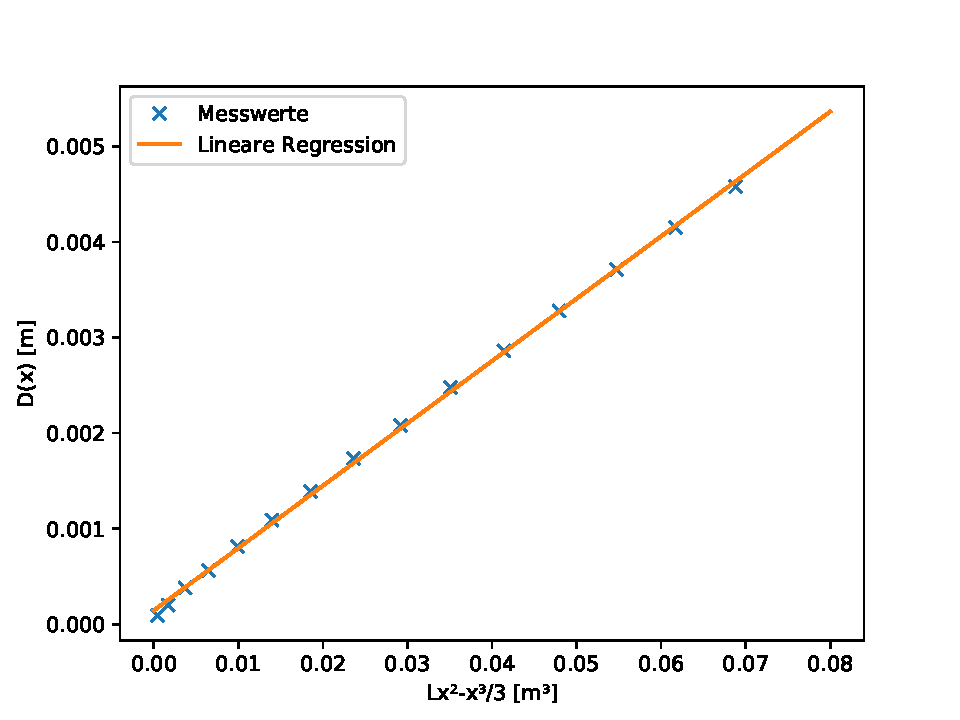
\includegraphics[width=0.7\linewidth]{reins.pdf}
        \caption{In der Grafik sind die Auslenkungen D gegen Lx²-x³/3 aufgetragen. Durch diese Wertepaare wurde zudem per linearer Regression eine Ausgleichsgerade gelegt. Deren Steigung beträgt 0,06525698 und deren y-Achsenabschnitt 0,00014415.}
        \label{fig:graphReins}
      \end{figure}

      Der Elastizitätsmodul des Materials wird nun analog zum eckigen Stab bei einseitiger Aufhängung mit $L = 0,49 $ und $m = 1,2082 kg$ bestimmt. Daraus ergibt sich wieder mit Gauß'scher Fehlerfortpflanzung:
      \begin{equation*}
        E_1 = 308,3912 \pm 2,2898 GPa \quad \text{mit } \Delta a = \pm 4,8454 \cdot 10^{-4} Pa
      \end{equation*}

      %\newpage

      \begin{table}[h]
        \centering
        \caption{Messwerte des runden, zweiseitig eingespannten Stabes wie in Tabelle \ref{tab:tabEzwei}.}
        \label{tab:tabRzwei}
        \begin{tabular}{c c c c c}
          \toprule
          {$x$ [m]} & {$D_0(x)$ [$10^{-3}m$]} & {$D_a(x)$ [$10^{-3}m$]} & {$D(x)$ [$10^{-3}m$]} & {$x_{rel}$ [m]}\\
          \midrule
          0.03 & 0.28 & 0.40 & 0.12 & 0.03\\
          0.06 & 0.41 & 0.65 & 0.24 & 0.06\\
          0.09 & 0.42 & 0.85 & 0.43 & 0.09\\
          0.12 & 0.41 & 0.97 & 0.56 & 0.12\\
          0.15 & 0.37 & 1.05 & 0.68 & 0.15\\
          0.18 & 0.26 & 1.12 & 0.86 & 0.18\\
          0.21 & 0.24 & 1.08 & 0.84 & 0.21\\
          0.24 & 0.19 & 1.07 & 0.88 & 0.24\\
          0.30 & 0.70 & 1.81 & 1.11 & 0.25\\
          0.33 & 0.61 & 1.68 & 1.07 & 0.22\\
          0.36 & 0.55 & 1.52 & 0.97 & 0.19\\
          0.39 & 0.49 & 1.34 & 0.85 & 0.16\\
          0.42 & 0.42 & 1.16 & 0.74 & 0.13\\
          0.45 & 0.34 & 0.96 & 0.62 & 0.10\\
          0.48 & 0.25 & 0.75 & 0.50 & 0.07\\
          0.51 & 0.16 & 0.50 & 0.34 & 0.04\\
          0.54 & 0.04 & 0.29 & 0.25 & 0.01\\
          \bottomrule            
        \end{tabular}
      \end{table}

      \begin{figure}[h]
        \centering
        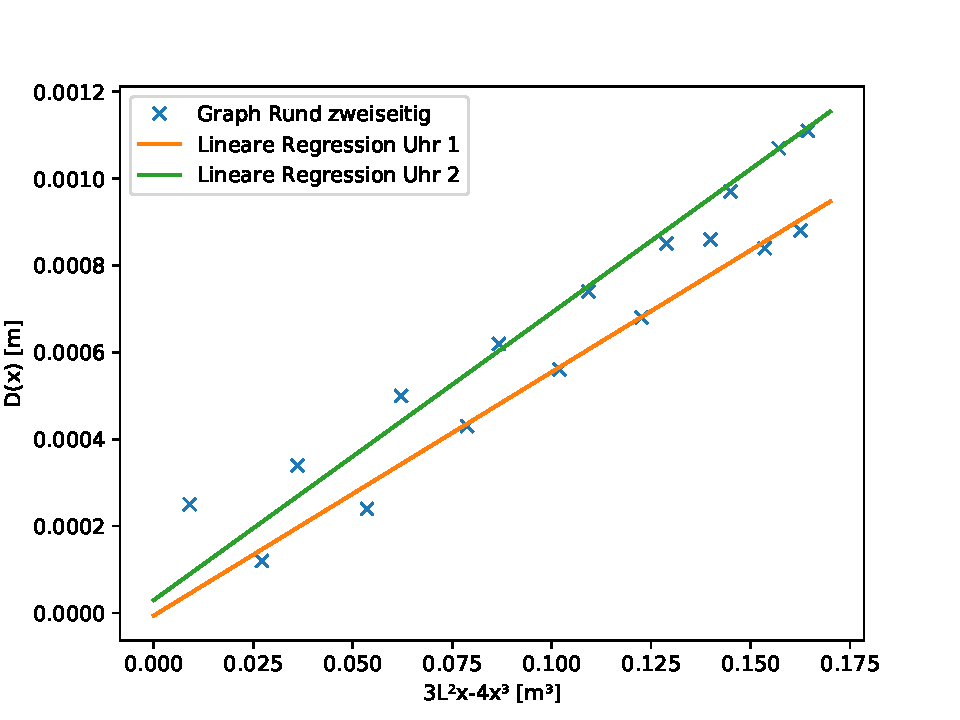
\includegraphics[width=0.7\linewidth]{rzwei.pdf}
        \caption{In der Grafik sind die Auslenkungen D gegen Lx²-x³/3 aufgetragen. Durch diese Wertepaare wurde zudem per linearer Regression zwei Ausgleichsgerade gelegt. Es wurden zwei Ausgleichsgeraden generiert, da die zwei Uhren stark unterschiedlich gemessen haben. Die Gerade von Uhr 1 hat die Steigung $5,60760\cdot10^{-3}$ und den y-Achsenabschnitt $-5,94841\cdot10^{-6}$, die von Uhr 2 die Steigung $6,61459\cdot10^{-3}$ und den y-Achsenabschnitt $2,98337\cdot10^{-5}$.}
        \label{fig:graphRzwei}
      \end{figure}
      Auch hier wird das Elastizitätsmodul analog zum Vorgang beim eckigen Stab bei zweiseitiger Auflage bestimmt. $L$ beträgt,
      wie beim eckigen Stab 0,55 m und $m$ ist ebenfalls 2,3679.
      \begin{equation*}
        \Delta a = (\Delta a_1 + \Delta a_2) \cdot \frac{1}{2} = 1,5896 \cdot 10^{-4}
      \end{equation*}
      \begin{equation*}
        E_2 = \frac{mg}{2mI} = 268,9202 \pm 6,9952 GPa \quad \text{mit } \Delta a = \pm 1,5896 \cdot 10^{-4}
      \end{equation*}

      Zunächst wird die Abweichung der im Experiment bestimmten Elastizitätsmodule berechnet. $E_2$ weicht um 12,7 \% von $E_1$ ab.
      Von dem Literaturwert [5, S.624], der 145GPa beträgt, weicht $E_1$ um 112,68 \% und $E_2$ um 85,4 \% ab.

      \FloatBarrier

    \newpage

    \section{Diskussion}
    Der Elastizitätsmodul, welcher aus den linearen Regressionen der Auslenkungen bei Einspannung des eckigen Stabes bestimmt wurde,
    weicht mit einem kleinen Fehler von dem Literaturwert ab, sodass es sich bei dem Stabmaterial wohl tatsächlich um
    Kupfer handelt. Die Genauigkeit dieser Messung könnte an der flachen Auflagefläche des Stabes, auf dem der Tastkopfes 
    der Messuhr auflag. Die vorhandenen Abweichungen sind vermutlich daraufhin zurückzuführen, dass die Messuhren sehr
    empfindlich waren und die Stäbe schon nicht lineare Anfangsauslenkungen aufgewiesen haben. Viel größere Abweichungen von
    den Literaturwerten sind bei der Einspannung des runden Stabes festzustellen. Der wahrscheinliche Grund der großen Abweichungen
    liegt in der gebogenen Oberfläche des Stabes, auf der der Tastkopf aufliegt. Durch horizontale Auslenkung des Stabes aus 
    vorherigen Versuchen liegt der Tastkopf nicht immer an der höchsten Stelle des Stabes auf und die Messwerte variieren stark.
    Hinzu kommt bei den Messungen mit zweiseitiger Einspannung, dass eine der beiden Messuhren im Vergleich zur anderen Uhr
    variierende Werte geliefert hat. Dies lag nach äußerer Betrachtung an der nicht stabilen Befestigung der 2. Uhr.
    Trotz der großen Abweichungen bei der Messung des Elastizitätsmoduls des runden Stabes, lässt sich das Elastizitätsmodul
    über den Literaturwert verifizieren, wenn die großen Fehlerquellen bei der Messung in Betracht gezogen werden.

    \newpage

    \section{Literaturverzeichnis}
      [1] \textit{Versuchsanleitung V103 - Biegung elastischer Stäbe.} TU Dormund, 2019
      [2] N. N. Greenwood, A. Earnshaw: \textit{Chemie der Elemente. 1. Auflage.} VCH, Weinheim 1988
      [3] Harry H. Binder: \textit{Lexikon der chemischen Elemente – das Periodensystem in Fakten, Zahlen und Daten.} S. Hirzel Verlag, Stuttgart 1999
      [4] TU München: \textit{Baustoffsammlung der Fakultät für Architektur der TU München} 02.Dezember.2019.
          \url{http://www.erlacher.net/wdb/metalle.php?doctype=2&id=6&gruppe=6} \newline
      [5] Horst Kuchling: \textit{Taschenbuch der Physik.} Carl Hanser, 2011
    
\end{document}